\section*{Chapter 19: Generative Models}
Given data coming from unknown distribution $p(x)$, learn $p_\theta(x)$ so that they are indistinguishable. Main challenges: mode collapse $p(x) >> p_\theta(x) \gtrapprox 0$ (all images look the same) and incorrect data $p_\theta(x) >> p(x) \gtrapprox 0$.

\subsection*{Generative Adversarial Networks}
Transform density estimation into classification. Idea: discriminator (D) cannot distinguish between true and generated samples by G:

$\tilde p_\theta(\x, y) = \frac{1}{2}(yp(\x) + (1-y)p_\theta(\x))$

\textbf{Bayes optimal classifier:} $q_\theta(x) = \frac{p(\x)}{p(\x) + p_\theta(\x)}$

Train generator by min logistic likelihood: $\theta \xMapsto[]{\min} l^*(\theta) := \E_{\tilde p_\theta} [y\ln q_\theta(\x) + (1-y)\ln(1-q_\theta(\x))]$

The objective that gets minimized is:

$\min_G\max_D L(D, G) = \E_{\mathbf x \sim p(\mathbf x)}[\log D(x)] + \E_{\mathbf z \sim p_\theta(\mathbf z)}[\log (1-D(z))]$ aka

$\E_{\frac{1}{2}(p+p_\theta)}[y\ln q_\theta(\x) + (1-y)\ln (1-q_\theta(\x))] = \E_{\frac{1}{2}(p+p_\theta)}[y\ln p(\x) + (1-y)\ln p_\theta(\x) - \ln(p(\x) + p_\theta(\x))] = -\frac{1}{2}H(p) -\frac{1}{2}H(p_\theta) + H(\frac{1}{2}(p+p_\theta))-\ln 2 = \text{JS}(p, p_\theta) - \ln 2 \to$ Jensen-Shannon div

Optimal class. is inaccesible, use NN $q_\phi : \x \to [0; 1]$

Define new objective via bound

$l^*(\theta) \geq \sup_{\phi\in\Phi} l(\theta, \phi)$

$l(\theta, \phi) := \E_{\tilde p_\theta}[y\ln q_\phi(\x) + (1-y)\ln(1-q_\phi(\x))]$

$\to \theta^* := \argmin_{\theta\in\Theta}\{\sup_{\phi\in\Phi}l(\theta, \phi)\}$

Use SGD (may diverge): $\theta^{t+1} = \theta^t - \alpha\nabla_\theta l(\theta^t, \phi^t)$

$\phi^{t+1} = \phi^t - \alpha\nabla_\phi l(\theta^{t+1}, \phi^t)$

Common trade-off: noisy samples but adequate representation of variability or faithful samples but lack of representation (mode dropping).

\subsection*{Normalizing flows}
Not as powerful as other generative models but they provide the likelihood. Goal: go from simple dist to complex and viceversa.

\textbf{Change of variable formula}. For a given RV $Z$ and $\x=g_\theta(z) \to p_X(\x) = p_Z(z) |\det(\frac{\partial g_\theta(z)}{\partial z^\top})|^{-1}$

or where $f_\theta(\cdot) = g_\theta(\cdot)^{-1}$: 

$p_X(\x) = p_Z(f(x))|\det(\frac{\partial f_\theta(x)}{\partial x^\top})|$

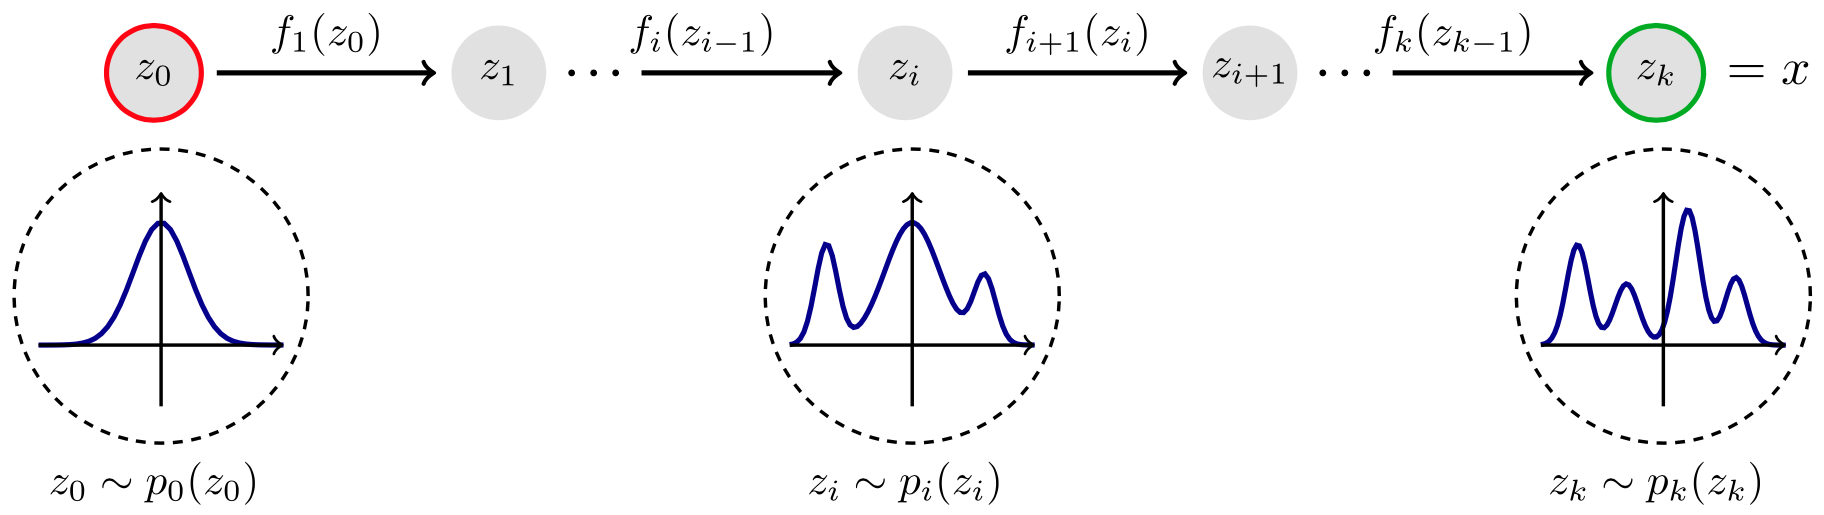
\includegraphics[width=\columnwidth]{src/normflows.png}

Normalizing flow is a bijection $F$ which is convenient to compute, invert and calculate $|\det(\partial F)|$. We use a stack of layers such that: 

- $F = F_L \circ \hdots \circ F_1$, $F^{-1} = F_1^{-1} \circ \hdots \circ F_L^{-1}$

- $\det(\partial F) = \prod_{l=1}^L \det(\partial F_l \circ \partial F_{l-1: 1})$

- $\det(\partial F^{-1}) = \det(\partial F)^{-1}$

- $\log p(\x|\z) = -\sum_{l=1}^L \log|\det(\partial F_l \circ F_{1:l-1})|$

\textbf{Linear flow}

Linear transform w/ invertible $A$: $F(z) = Az + b$, $\partial F = A$. It is equal to linear factor analysis if $z \sim N(0, \mathbb{I})$. Requires $O(n^3)$ to compute det and inv.

\textbf{(Tri-)Diagonal flows}. They use a diagonal matrix as $A$. In Triagonal, $A$ is upper or lower triagonal. Complexity decays but not very powerful.